%------------------------------------------------------------------------------------------------------------------------
\chapter{現行ピクセルモジュールの電荷較正}
\label{sec:chap3}
%------------------------------------------------------------------------------------------------------------------------

FEチップから得られるToT(Time over Threshold)を荷電粒子がシリコンセンサーに落とす電荷に較正する必要がある。本章では、電荷較正のための試験電荷生成回路の詳細について説明し、その後に電荷較正手法について述べる。

%------------------------------------------------------------------------------------------------------------------------
\section{アナログ回路}
\label{sec:analog}
%------------------------------------------------------------------------------------------------------------------------
\fref{fig:analog}にFEI3のアナログ回路の概略図を示す。センサーにおいて生成された電子をFEチップにおいて検知するために、バンプにより接合されている。内部電位によりバンプに向かってドリフトした電子を検出し、バンプの接合部からFEチップへ送りプリアンプで整形および増幅を行う。キャパシタ$C_\mathrm{F}$は信号により充電され、電荷量に依らない一定のフィードバック電流によって放電される。\fref{fig:analog}の$8\ \si{bit}$のIF DACによってFEチップ全体のピクセルについてのフィードバック電流の増幅率の調整を行い、$3\ \si{bit}$のFDACを用いてピクセルごとのフィードバック電流の増幅率の調整を行う。これにより、バンプからの信号は\fref{fig:sannkakuha}のようになり、この三角波の波高は入射電荷量によって決定される。整形および増幅された信号をToTにデジタル変換し、後段のフレキシブル基板へ信号を送る。

一方で、Thresholdの測定や電荷較正のために用いる電荷はFEチップ内の回路で生成する。FEチップにおいて試験電荷を生成するために、電圧$V_\mathrm{cal}$を自由に設定できる回路と2つのキャパシタ$C_\mathrm{low}, C_\mathrm{high}$が搭載されている。試験電荷生成のために、$C_\mathrm{low}=8\ \si{fF}$のキャパシタを用いる場合と、$C_\mathrm{low}+C_\mathrm{high}=40\ \si{fF}$の合成キャパシタを用いる場合がある。$C_\mathrm{low}+C_\mathrm{high}$の合成キャパシタを用いる場合は生成した試験電荷から得られるToTが約$10\%$小さく出力されることがわかっている。そのため、Thresholdの測定や電荷較正を行う際には、$C_\mathrm{low}$のキャパシタを用いて試験電荷の生成を行う。

\begin{figure}[tbp]
  \centering
  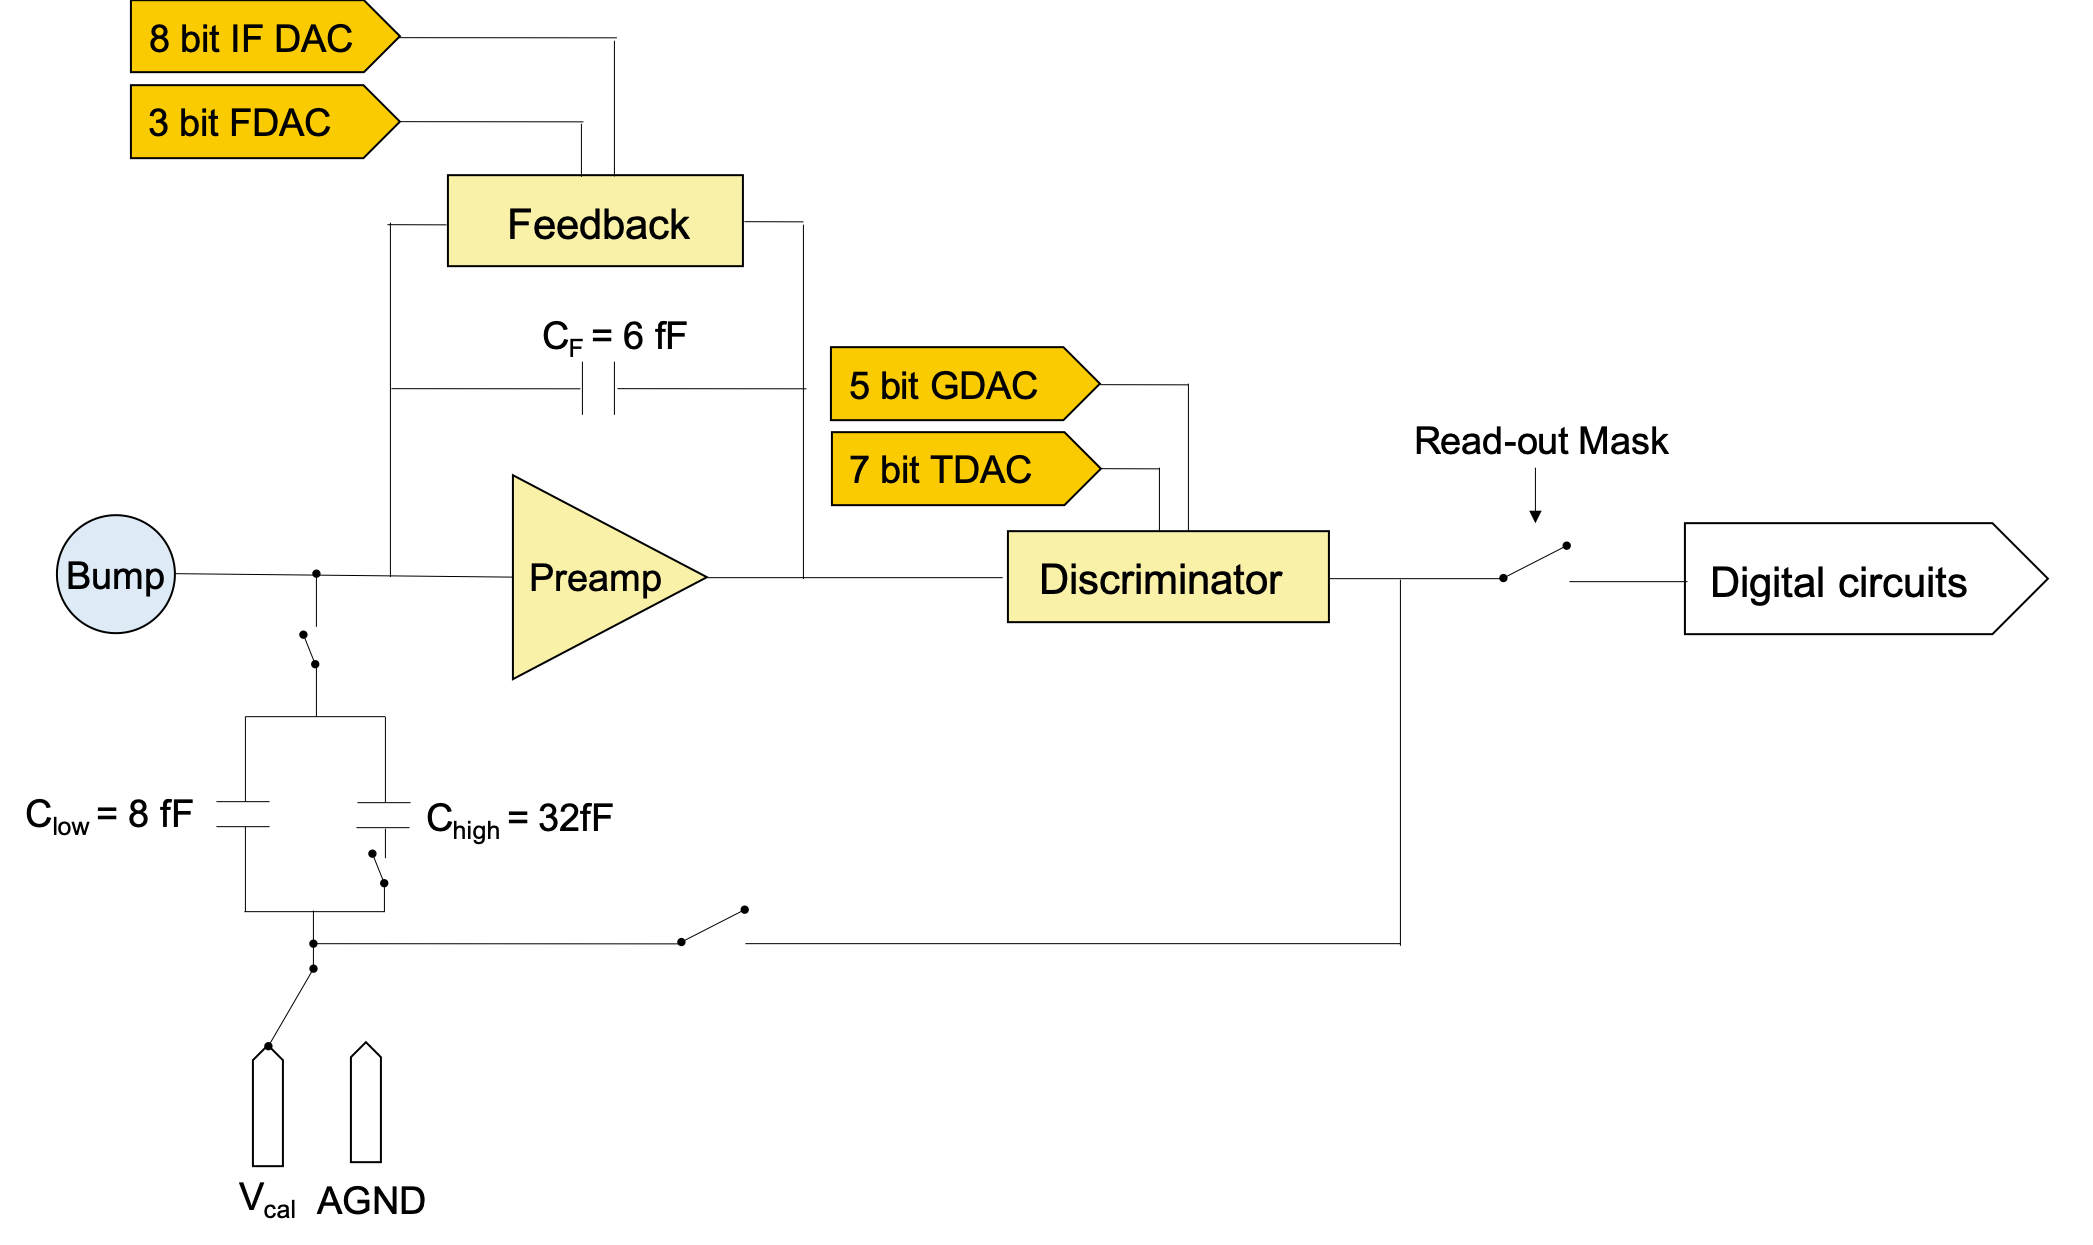
\includegraphics[height=9cm,keepaspectratio]{analog2.png}
  \caption[FEI3アナログ回路の概略図]{FEI3アナログ回路の概略図。電荷較正やThresholdスキャンのための試験電荷は$V_\mathrm{cal}$とキャパシタ($C_\mathrm{low},\ C_\mathrm{high}$)の組み合わせによって生成される。}
  \label{fig:analog}
\end{figure}

\begin{figure}[tbp]
  \centering
  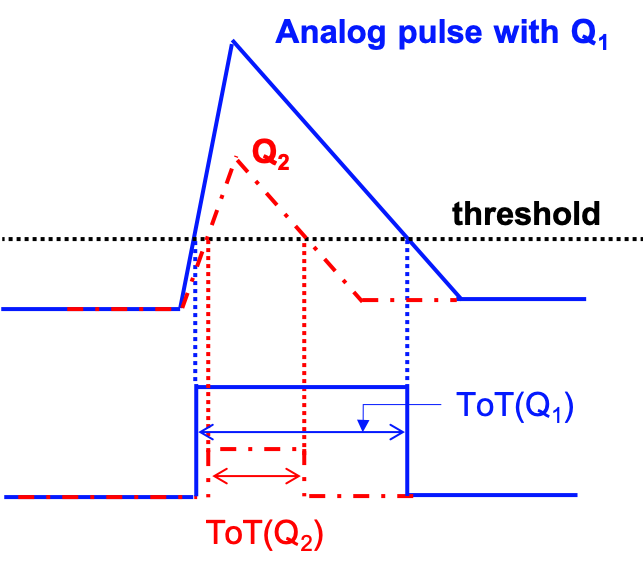
\includegraphics[height=6cm,keepaspectratio]{calibeq2.png}
  \caption[ToTと荷電粒子がシリコンセンサーに落とす電荷量$Q$の概念図]{ToTと荷電粒子がシリコンセンサーに落とす電荷量$Q$の概念図。図中の青線と赤線はある電荷量$(Q_1>Q_2)$がToTに変換される概念図である。図中上半分の三角波はアナログ回路のフィードバック回路にて整形・増幅された信号であり、その信号がThreshold値を超える時間であるToTに変換される。三角波立ち上がりはピークまでに約$40\ \si{ns}$になるよう調整されるため電荷量により傾きが異なるが、立ち下がりはフィードバック回路によって制御されるため、電荷量に依存せず一定の傾きである。}
  \label{fig:sannkakuha}
\end{figure}



%------------------------------------------------------------------------------------------------------------------------
\section{電荷較正手法}
\label{sec:calibway}
%------------------------------------------------------------------------------------------------------------------------
ピクセルモジュールの出力であるToTを較正し、荷電粒子が落とした電荷量に変換する方法について説明する。各ピクセル間の差異を少なくするために、ToTの較正を行う前に、ThresholdやToTを目標値になるようチューニングを行う必要がある。以下ではチューニングと電荷較正の方法について説明する。


%------------------------------------------------------------------------------------------------------------------------
\subsection{チューニング}
\label{sec:tuning}
%------------------------------------------------------------------------------------------------------------------------
各ピクセルにおけるThresholdと、ある基準電荷量の信号に対するToTを任意の値に調整するためにFEチップのチューニングを行う。Run2におけるThresholdおよびMIP相当の参照電荷量に対応するToTの目標値をそれぞれ\tref{tab:thresholdtuning}、\tref{tab:tottuning}に示す。さらに、2022年3月から始まるRun3では、B-LayerのThresholdは$3500\ \si{e}$でありToTのチューニングは$20\ \si{ke}$の電荷に対して$18\ \si{ToT}$、IBLのThresholdは$1500\ \si{e}$でありToTのチューニングは$16\ \si{ke}$の電荷に対して$10\ \si{ToT}$である。

\begin{table}[tbp]
  \begin{center}
    \caption[各LayerにおけるThresholdの値]{各LayerにおけるThresholdの目標値。}
    \label{tab:thresholdtuning}
    \begin{tabular}{|l||r|r|r|r|}
    \hline
      Layer名  & 2015年($4\ \si{fb^{-1}}$) & 2016年($39\ \si{fb^{-1}}$) & 2017年($50\ \si{fb^{-1}}$) & 2018年($63\ \si{fb^{-1}}$) \\
    \bhline{1.5pt}
      IBL & $2500$ & $2500$ & $2500$ & $2000$ \\
    \hline
      B-Layer(中央) & $3500$ & $3500$ & $5000$ & $4300$ \\
    \hline
      B-Layer(前方) & $3500$ & $3500$ & $5000$ & $5000$ \\
    \hline
      Layer1 & $3500$ & $3500$ & $3500$ & $3500$ \\
    \hline
      Layer2 & $3500$ & $3500$ & $3500$ & $3500$ \\
    \hline
      Disk & $3500$ & $3500$ & $4500$ & $3500$ \\
    \hline
    \end{tabular}
  \end{center}
\end{table}


\begin{table}[tbp]
  \begin{center}
    \caption[各LayerにおけるToTのチューニングの値]{各LayerにおけるToTの目標値。表中における括弧はToTに対する電荷量であり、この値はMIP粒子がセンサーに落とす電荷量を表す。}
    \label{tab:tottuning}
    \begin{tabular}{|l||r|r|r|r|}
    \hline
      Layer名  & 2015年($4\ \si{fb^{-1}}$) & 2016年($39\ \si{fb^{-1}}$) & 2017年($50\ \si{fb^{-1}}$) & 2018年($63\ \si{fb^{-1}}$) \\
    \bhline{1.5pt}
      IBL & $10 \mathrm{ToT} (16\ \si{ke})$ & $8 \mathrm{ToT} (16\ \si{ke})$ & $8 \mathrm{ToT} (16\ \si{ke})$ & $10 \mathrm{ToT} (16\ \si{ke})$ \\
    \hline
      B-Layer & $30 \mathrm{ToT} (20\ \si{ke})$ & $18 \mathrm{ToT} (20\ \si{ke})$ & $18 \mathrm{ToT} (20\ \si{ke})$ & $18 \mathrm{ToT} (20\ \si{ke})$ \\
    \hline
      Layer1 & $30 \mathrm{ToT} (20\ \si{ke})$ & $30 \mathrm{ToT} (20\ \si{ke})$ & $30 \mathrm{ToT} (20\ \si{ke})$ & $30 \mathrm{ToT} (20\ \si{ke})$ \\
    \hline
      Layer2 & $30 \mathrm{ToT} (20\ \si{ke})$ & $30 \mathrm{ToT} (20\ \si{ke})$ & $30 \mathrm{ToT} (20\ \si{ke})$ & $30 \mathrm{ToT} (20\ \si{ke})$ \\
    \hline
      Disk & $30 \mathrm{ToT} (20\ \si{ke})$ & $30 \mathrm{ToT} (20\ \si{ke})$ & $30 \mathrm{ToT} (20\ \si{ke})$ & $30 \mathrm{ToT} (20\ \si{ke})$ \\
    \hline
    \end{tabular}
  \end{center}
\end{table}

チューニングには、あるFEチップにおける全ピクセルのTresholdと任意の値に対するToTを調整するためのglobalチューニングと各ピクセルごとの値を目標値に近づけるlocalチューニングがある。はじめに、globalチューニングを行い、\fref{fig:analog}におけるIF DACおよび$5\ \si{bit}$のGDAC(\textbf{G}lobal \textbf{DAC})の値を調整し全ピクセルのThresholdまたはToTを大まかに目標値に合わせる。この段階では、全ピクセルから得られるThreshold分布およびToT分布の分散は大きいため、localチューニングを行い、\fref{fig:analog}におけるFDACおよび$7\ \si{bit}$のTDAC (\textbf{T}rim \textbf{DAC})の値を調整することにより各ピクセルが返す値を目標値にさらに近づける。
%ToTの値はThresholdに依存するため、Thresholdのチューニングの前後においてToTが変わってしまう。また、同様にToTチューニングの後はThreshold値が変化してしまう。この影響は、チューニングを繰り返すことで小さくなり、

チューニングの後、ThresholdスキャンやToTスキャンを行い各ピクセルにおける値を測定する。ThresholdスキャンおよびToTスキャンの方法を以下に述べる。

%------------------------------------------------------------------------------------------------------------------------
\subsubsection{Thresholdスキャン}
\label{sec:thresholdscan}
%------------------------------------------------------------------------------------------------------------------------
Thresholdスキャンでは、各ピクセルに試験電荷を入射しThresholdとノイズを測定する。試験電荷を増加させつつ検出効率を測定し、\fref{fig:threshold}に示す様な分布を作成する。この分布はS字を描くため、\textbf{Sカーブ}と呼ばれている。\fref{fig:threshold}中の青線はSカーブのフィッティングであり、\eref{eq:gosakannsuu}のような誤差関数を用いて定義される。
\begin{equation}
  \label{eq:gosakannsuu}
  f(x)=0.5\times\left[ 2-\mathrm{erfc}\left( \frac{x-Q_\mathrm{threshold}}{\sigma \times \sqrt{2}} \right)  \right]
\end{equation}
Sカーブにおいて、検出効率が$50\%$となる試験電荷の値をThresholdと定義し、検出効率が$16.5\%$と$83.5\%$となる試験電荷の幅をノイズと定義する。

\begin{figure}[tbp]
  \centering
  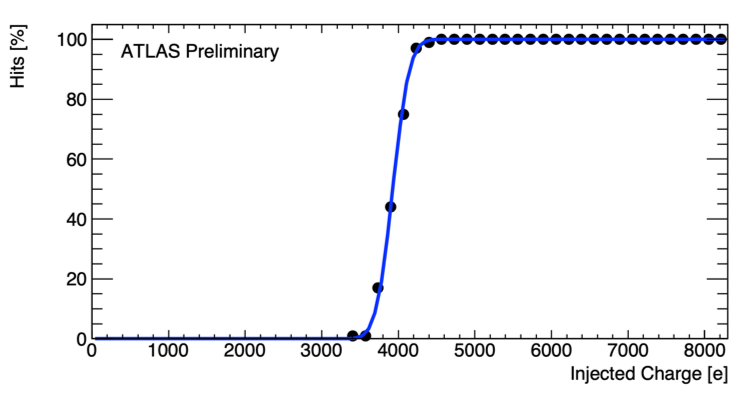
\includegraphics[height=7cm,keepaspectratio]{threshold.png}
  \caption[検出効率と試験電荷の関係]{検出効率と試験電荷の関係 \cite{calibnoise}。黒点はある試験電荷に対する応答率の測定点であり、青線は\eref{eq:gosakannsuu}によるフィッティング結果を表す。検出効率が$50\%$となる試験電荷の値がThresholdであり、検出効率が$16.5\%$と$83.5\%$となる試験電荷の幅がノイズである。}
  \label{fig:threshold}
\end{figure}


%------------------------------------------------------------------------------------------------------------------------
\subsubsection{ToTスキャン}
\label{sec:totscan}
%------------------------------------------------------------------------------------------------------------------------
ToTスキャンでは、一定の試験電荷を各ピクセルに100回入射させ、その試験電荷に対するToTの値の測定を行う。各ピクセルから得られるToTの値はデジタル値であるため整数値であるが、100回のスキャンの平均値をある試験電荷に対するToTとするため、この値は小数値を取り得る。


%------------------------------------------------------------------------------------------------------------------------
\subsection{電荷較正}
\label{sec:calibration}
%------------------------------------------------------------------------------------------------------------------------
\ref{sec:ASIC}節で示した様に、原理的にはToTと荷電粒子がシリコンセンサーに落とす電荷量$Q$は線形関係になると予想される。しかし、実際にはタイムウォーク等の二次的な効果を受け、線形関係ではなくなってしまう。\fref{fig:calibnijikouka}に、タイムウォークの影響が大きくなる小さい電荷量について、パルスの立ち上がり点をずらした際のToTの変化の様子を示す。タイムウォークの影響が大きくなる電荷量について、パルスの立ち上がり点がずれるとThresholdを超えるクロックウィンドウが1つ後ろにずれてしまうことが発生しやすくなり、小さいToTを出力する割合が増える。そのため、小さい電荷量におけるToTスキャンでは、原理的に予想されるToTと比べて平均的なToTが小さくなる。さらに、タイムウォークによりパルスの立ち上がりの傾きが電荷量によって異なることから、小さい電荷量においてToTと電荷量の関係は線形ではなくなると考えられる。

このような二次的な効果を含めた電荷較正式は、\eref{eq:calibration}のように表される。
\begin{equation}
  \label{eq:calibration}
  \mathrm{ToT} = p_0\frac{p_1 + Q}{p_2 + Q}
\end{equation}
\eref{eq:calibration}に示した3つのパラメータを求めるために、\fref{fig:analog}に示したアナログ回路の$V_\mathrm{cal}$の値を変えることにより電荷量を変化させつつ試験電荷を入射し、ToTの較正を行う。電荷較正は各ピクセルに対してパラメータを求めるのではなく、FEチップごとに一律の値を用いる。そのため、ToTスキャンから得られたピクセルごとのToTの平均値を用いてFEチップに対する電荷較正を行う。

%\begin{figure}[tbp]
%  \begin{minipage}[b]{0.5\linewidth}
%    \centering
%    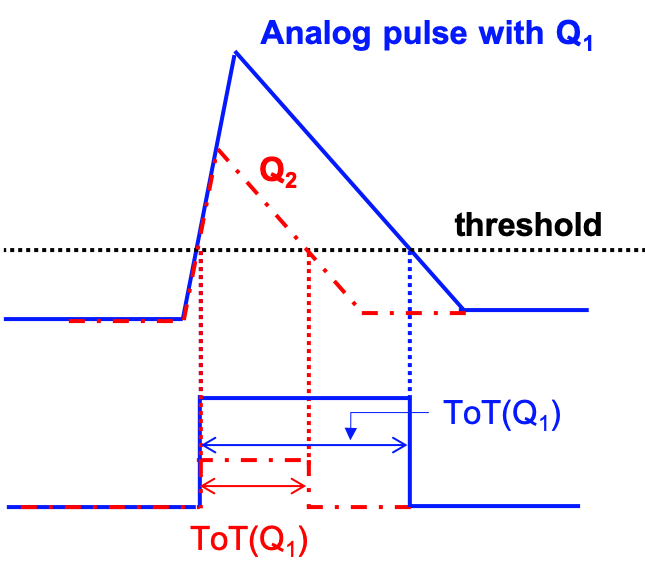
\includegraphics[keepaspectratio, scale=0.6]{calibeq1.png}
%  \end{minipage}
%  \begin{minipage}[b]{0.5\linewidth}
%    \centering
%    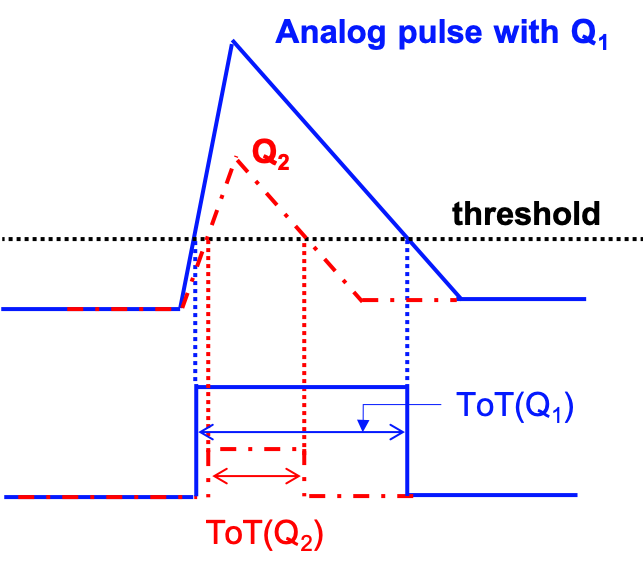
\includegraphics[keepaspectratio, scale=0.6]{calibeq2.png}
%  \end{minipage}
%  \caption[ToTと荷電粒子がシリコンセンサーに落とす電荷量$Q$の概念図]{ToTと荷電粒子がシリコンセンサーに落とす電荷量$Q$の概念図。図中の青線と赤線はある電荷量$(Q_1>Q_2)$がToTに変換される概念図である。左図はToTと電荷量$Q$の関係が理想的に線形になる場合で、右図はタイムウォーク等の二次的な効果を受けた場合の図である。図中上半分の三角波はアナログ回路のフィードバック回路にて整形・増幅された信号であり、その信号がThreshold値を超える時間であるToTに変換される。三角波の立ち上がりはタイムウォークによって変化するが、立ち下がりはフィードバック回路によって制御されるため、電荷量に依存せず一定の傾きである。}
%  \label{fig:calibnijikouka}
%\end{figure}

\begin{figure}[tbp]
  \centering
  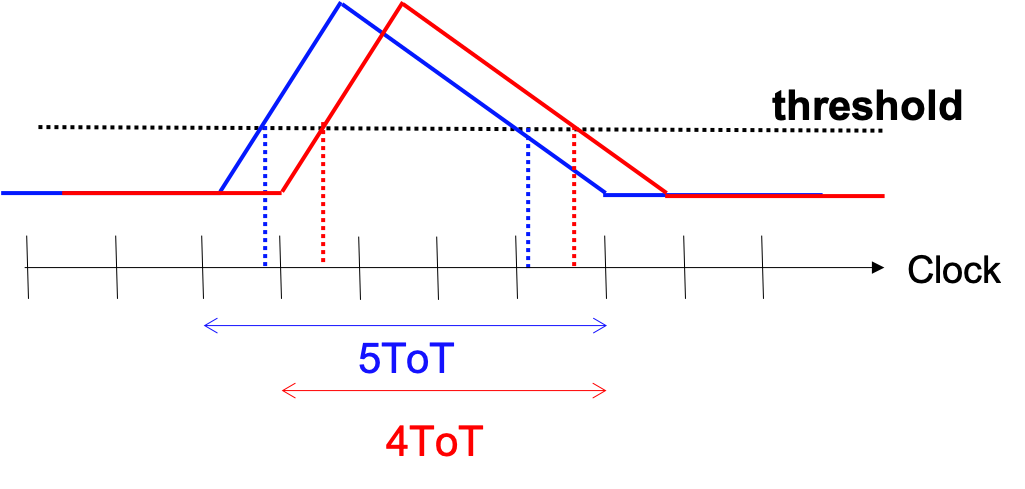
\includegraphics[height=5cm,keepaspectratio]{timewalklowtot.png}
  \caption[同じ電荷量のアナログ信号においてパルスの立ち上がり点をずらした際のToTの変化]{同じ電荷量のアナログ信号においてパルスの立ち上がり点をずらした際のToTの変化の様子。タイムウォークの影響が大きくなる電荷量に対しては、小さいToTを出力することが多くなる。}
  \label{fig:calibnijikouka}
\end{figure}

FEI4を用いているIBLについてはToTの出力が4bitと少ないことから、Run3からは\eref{eq:calibration}によるフィッティングは行わず、ToTの値と試験電荷の値の対応情報を持つルックアップテーブルを用いて較正を行う。本研究では\eref{eq:calibration}を用いた電荷較正手法について取り扱うため、以下ではFEI3を用いている現行のピクセル検出器の電荷較正のみについて述べる。

%------------------------------------------------------------------------------------------------------------------------
\section{電荷較正結果の履歴}
\label{sec:probrem}
%------------------------------------------------------------------------------------------------------------------------
Thresholdのチューニングや電荷較正を行った後、それらに関する情報はCERNに設置されているデータベース\cite{pixeldb}に保存する必要がある。このデータベースでは電荷較正に関する情報や検出器の配置や温度等のDCS(Data Control System)情報、さらにトリガー情報等を保管する。これらの情報は、測定におけるイベント選別やモンテカルロシミュレーションのためのイベント作成等に用いられる。

ThresholdスキャンおよびToTスキャンは各ピクセルごとの値を出力するが、データベースへはあるFEチップにおけるThresholdの平均値およびToTの平均値を用いた電荷較正式(\ref{eq:calibration})のパラメータのみを登録する。また、各ピクセルの大部分は\tref{tab:asicsiyou}に示した構造をしているが、FEチップの境界付近では不感領域をなるべく少なくするために、構造の異なったピクセルを配置する。FE-I3の境界付近におけるピクセルの構造を\fref{fig:pixeltypes}に示す。\tref{tab:asicsiyou}に示した通常のピクセルのことをnormalピクセル(図中の青の領域)と呼び、黄色の領域のピクセルをlongピクセル、赤色の領域をgangedピクセルと呼ぶ。
normalピクセルの大きさは$50\times 400\ \si{\micro m^2}$であるのに対して、longピクセルは$50\times 600\ \si{\micro m^2}$であり、長方形の一辺の長さがnormalピクセルの1.5倍となっている。また、gangedピクセルはnormalピクセル2つをワイヤーで接続した構造をしている。このような構造の違いから、ノイズ等の値が異なる値になるため、データベースへはそれぞれの値をアップロードする。


\begin{figure}[tbp]
  \centering
  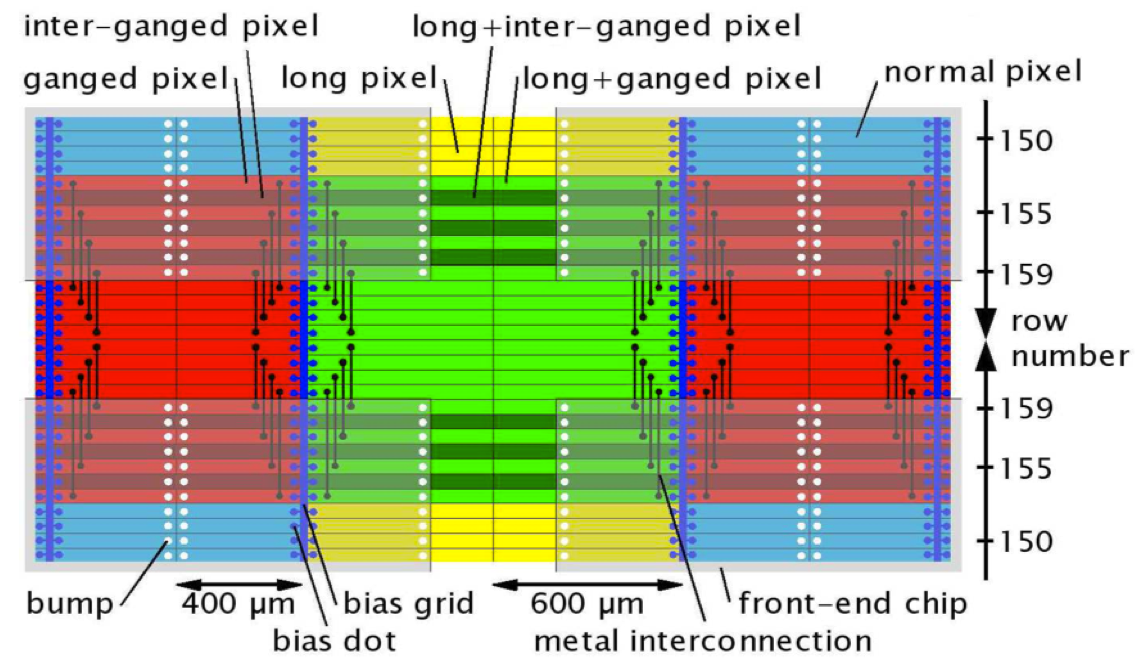
\includegraphics[height=6cm,keepaspectratio]{pixeltypes2.png}
  \caption[ピクセルモジュールのFEチップ境界付近のピクセルタイプ]{ピクセルモジュールのFEチップ境界付近のピクセルタイプ \cite{pixeltypes}。FE-I3は$160\times18$ [行$\times$列]のピクセルを持ち、$2\times8$ [行$\times$列]のFE-I3を並べて1つのピクセルモジュールを構成する。FE-I3の1列目および18列目がlongピクセル、$154,\ 156,\ 158,\ 160$列目がgangedピクセルと定義される。2つのgangedピクセルの間にはinter-gangedピクセルというピクセルが存在するが、ノイズ等の特性はnormalピクセルと同等の値を持つ。}
  \label{fig:pixeltypes}
\end{figure}

データベースに登録する情報を以下に示す。
\begin{itemize}
  \item Thresholdの平均値
  \item Thresholdの分散
  \item Thresholdのノイズ
  \item In-time threshold
  \item 電荷較正式(\ref{eq:calibration})における3つのパラメータ
  \item 電荷較正におけるフィッティングの誤差
\end{itemize}




\newpage
